\documentclass{article}
\usepackage{tikz}
\usepackage{float}
\usepackage{enumerate}
\usepackage{amsmath}
\usepackage{amsthm}
\usepackage{bm}
\usepackage{indentfirst}
\usepackage{siunitx}
\usepackage[utf8]{inputenc}
\usepackage{graphicx}
\graphicspath{ {Images/} }
\usepackage{float}
\usepackage{mhchem}
\usepackage{chemfig}
\allowdisplaybreaks

\title{6.041 Problem Set 8}
\author{Robert Durfee - R02}
\date{October 31, 2018}

\begin{document}

\maketitle

\section*{Problem 1}

\subsection*{Part A}

The equation for the CDF of $Y$ is
$$ F_Y(y) = P(Y \leq y) $$
However, $Y$ can be written in terms of $X$, 
$$ P(Y \leq y) = P(e^X \leq y) $$
Rearranging terms,
$$ F_Y(y) = P(X \leq \ln y) $$
The right side is just the CDF for $X$, which is known, thus
$$ F_Y(y) = F_X(\ln y) $$
Taking the derivative to convert to PDF,
$$ f_Y(y) = \frac{1}{y} f_X(\ln y) $$

\subsection*{Part B}

Substituting the $f_X(x)$ into the equation from Part A,
$$ f_Y(y) = \begin{cases}
  1 / 3y & -2 < \ln y \leq 1 \\
  0 & \mathrm{otherwise}
\end{cases} $$
Simplifying
$$ f_Y(y) = \begin{cases}
  1 / 3y & e^{-2} < y \leq e \\
  0 & \mathrm{otherwise}
\end{cases} $$

\subsection*{Part C}

Substituting the $f_X(x)$ into the equation from Part A,
$$ f_Y(y) = \begin{cases}
  2 e^{-2 \ln y} / y & \ln y > 0 \\
  0 & \mathrm{otherwise}
\end{cases} $$
Simplifying
$$ f_Y(y) = \begin{cases}
  2 / y^3 & y > 1 \\
  0 & \mathrm{otherwise}
\end{cases} $$

\subsection*{Part D}

Substituting the $f_X(x)$ into the equation from Part A,
$$ f_Y(y) = \frac{1}{\sqrt{2 \pi} y} e^{-(\ln y)^2 / 2} $$

\section*{Problem 2}

\subsection*{Part A}

The CDF of $Z$ is given by
$$ F_Z(z) = P(Z \leq z) $$
However, $Z$ can be written in terms of $X$ and $Y$,
$$ P(Z \leq z) = P(\max\{X, Y\} \leq z) $$
Which is the same as
$$ P(Z \leq z) = P(\{X \leq z\} \cap \{Y \leq z\}) $$
Since both variables are independent,
$$ P(Z \leq z) = P(X \leq z) P(Y \leq z) $$
Therefore, written using known CDFs,
$$ F_Z(z) = F_X(z) F_Y(z) $$
Differentiating with respect to $z$,
$$ f_Z(z) = f_X(z) F_Y(z) + F_X(z) f_Y(z) $$
Since both $X$ and $Y$ are uniform over $[0, 1]$,
$$ F_X(x) = x,\, f_X(x) = \begin{cases}
  1 & x \in [0, 1] \\
  0 & \mathrm{otherwise}
\end{cases} $$
$$ F_Y(y) = y,\, f_Y(y) = \begin{cases}
  1 & y \in [0, 1] \\
  0 & \mathrm{otherwise}
\end{cases} $$
Therefore, the PDF of $Z$ is
$$ f_Z(z) = \begin{cases}
  2 z & z \in [0, 1] \\
  0 & \mathrm{otherwise}
\end{cases} $$

\subsection*{Part B}

The CDF of $Z$ is given the same as in Part A, except with a small change,
$$ F_Z(z) = P(2X \leq z) P(Y \leq z) $$
Moving the constant to the other side,
$$ F_Z(z) = P(X \leq z / 2) P(Y \leq z) $$
Written using known CDFs,
$$ F_Z(z) = F_X(z / 2) F_Y(z) $$
Differentiating with respect to $z$,
$$ f_Z(z) = f_X(z / 2) F_Y(z) / 2 + F_X(z / 2) f_Y(z) $$
Using the PDFs and CDFs from above, but noting that the PDF for $Y$ is $0$
when $z \in [1, 2]$, the PDF for $Z$ is
$$ f_Z(z) = \begin{cases}
  z & z \in [0, 1] \\
  1 / 2 & z \in [1, 2] \\
  0 & \mathrm{otherwise}
\end{cases} $$

\subsection*{Part C}

The CDF of $Z$ is given by
$$ F_Z(z) = P(Z \leq z) $$
However, $Z$ can be written in terms of $X$ and $Y$,
$$ P(Z \leq z) = P(\min\{X, Y\} \leq z) $$
Which is the same as
$$ P(Z \leq z) = 1 - P(\{X > z\} \cap \{Y > z\}) $$
Since both variables are independent,
$$ P(Z \leq z) = 1 - P(X > z) P(Y > z) $$
Therefore, written using known CDFs,
$$ F_Z(z) = 1 - (1 - F_X(z)) (1 - F_Y(z)) $$
Differentiating with respect to $z$,
$$ f_Z(z) = f_X(z) (1 - F_Y(z)) + (1 - F_X(z)) f_Y(z) $$
Using the PDFs and CDFs from above,
$$ f_Z(z) = \begin{cases}
  2 - 2z & z \in [0, 1] \\
  0 & \mathrm{otherwise}
\end{cases} $$

\section*{Problem 3}

\subsection*{Part A}

Using the discrete convolution,
$$ f_Z(z) = \sum_x p_X(x) p_Y(z - x) $$
The $x$ are in $\{0, 1, 2\}$ and $y$ in $\{3, 4\}$. Therefore, using the PDFs
given, the convolution becomes
$$ f_Z(z) = \begin{cases}
  1 / 6 & z = 3 \\
  2 / 6 & z = 4 \\
  2 / 6 & z = 5 \\
  1 / 6 & z = 6 \\
  0 & \mathrm{otherwise}
\end{cases} $$

\subsection*{Part B}

Using the continuous convolution,
$$ f_Z(z) = \int_z f_X(x) f_Y(z - x) dx $$
Given the PDFs, the range for $x$ is both $x \in [0, 2]$ and $x \in [z - 4, z
- 3]$ Therefore, the convolution becomes
$$ f_Z(z) = \int\limits_{\max\{z - 4, 0\}}^{\min\{z - 3, 2\}} f_X(x) f_Y(z -
x) dx $$
Substituting the values of the PDFs,
\begin{align*}
  f_Z(z) &= \int\limits_{\max\{z - 4, 0\}}^{\min\{z - 3, 2\}} \frac{1}{2} dx \\
  &= \left( \frac{x}{2} \right)_{\max\{z - 4, 0\}}^{\min\{z - 3, 2\}} \\
  &= \frac{1}{2}(\min\{z - 3, 2\} - \max\{z - 4, 0\})
\end{align*}
With proper bounds, this is
$$ f_Z(z) = \begin{cases}
  (\min\{z - 3, 2\} - \max\{z - 4, 0\}) / 2 & z \in [3, 6] \\
  0 & \mathrm{otherwise}
\end{cases} $$

\subsection*{Part C}

\begin{center}
    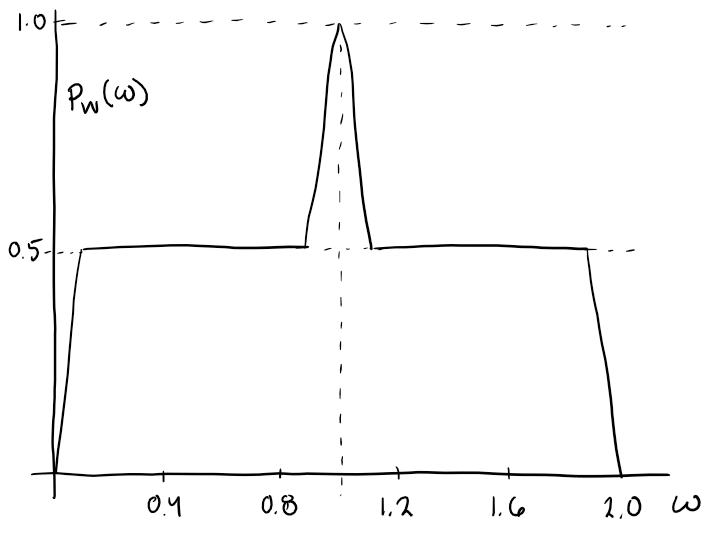
\includegraphics[scale=0.5]{Images/P3C.PNG}
\end{center}

\section*{Problem 4}

\subsection*{Part A}

The two events should be negatively correlated. The more times you roll $1$
in a fixed number of rolls, the fewer number of times you can roll a $2$.
This is true always and for all $i \neq j \in \{1, 2, \ldots, k\}$.

\subsection*{Part B}

The definition for covariance is 
$$ \mathrm{cov}(X_1, X_2) = E[X_1 X_2] - E[X_1] E[X_2] $$
To represent $X_1$ and $X_2$, use the sum of indicator random variables which
encode whether or not a $1$ or a $2$ was rolled on a given roll,
respectively. That is,
$$ X_1 = \sum_{i = 1}^n I_1^{(i)},\, X_2 = \sum_{j = 1}^n I_2^{(j)} $$
Then, the covariance can be written as
$$ \mathrm{cov}(X_1, X_2) = E\left[\sum_{i = 1}^n I_1^{(i)} \sum_{j = 1}^n
I_2^{(j)}\right] - E\left[\sum_{i = 1}^n I_1^{(i)}\right] E\left[\sum_{j =
1}^n I_2^{(j)}\right] $$
Given the linearity of expectation,
$$ \mathrm{cov}(X_1, X_2) = E\left[\sum_{i = 1}^n I_1^{(i)} \sum_{j = 1}^n
I_2^{(j)}\right] - \sum_{i = 1}^n E\left[I_1^{(i)}\right] \sum_{j = 1}^n
E\left[I_2^{(j)}\right] $$
Where the expectation of an indicator random variable is just the probability,
$$ \mathrm{cov}(X_1, X_2) = E\left[\sum_{i = 1}^n I_1^{(i)} \sum_{j = 1}^n
I_2^{(j)}\right] - \sum_{i = 1}^n p_1 \sum_{j = 1}^n p_2 $$
Reducing the sums,
$$ \mathrm{cov}(X_1, X_2) = E\left[\sum_{i = 1}^n I_1^{(i)} \sum_{j = 1}^n
I_2^{(j)}\right] - n^2 p_1 p_2 $$
Now, for the first term. This can be broken into two groups $i = j$ and $i
\neq j$
$$ \mathrm{cov}(X_1, X_2) = E\left[\sum_{i = j}^n I_1^{(i)} I_2^{(j)} +
\sum_{i \neq j}^n I_1^{(i)} I_2^{(j)}\right] - n^2 p_1 p_2 $$
However, it is impossible to roll a $1$ and a $2$ on the same roll, therefore
the first sum is equal to zero.
$$ \mathrm{cov}(X_1, X_2) = E\left[\sum_{i \neq j}^n I_1^{(i)}
I_2^{(j)}\right] - n^2 p_1 p_2 $$
Again, using linearity of expectation,
$$ \mathrm{cov}(X_1, X_2) = \sum_{i \neq j}^n E\left[I_1^{(i)}
I_2^{(j)}\right] - n^2 p_1 p_2 $$
The expectation of the indicator random variables is again the probability, thus
$$ \mathrm{cov}(X_1, X_2) = (n^2 - n) p_1 p_2 - n^2 p_1 p_2 = -n p_1 p_2 $$
Substituting the probability $1/k$ for both $p_1$ and $p_2$,
$$ \mathrm{cov}(X_1, X_2) = -\frac{n}{k^2} $$

\subsection*{Part C}

The work in Part B already gave a generalized answer
$$ \mathrm{cov}(X_1, X_2) = -n p_1 p_2 $$

\section*{Problem 5}

The equation for correlation coefficient is
$$ \rho(X, Y) = \frac{\mathrm{cov}(X,
Y)}{\sqrt{\mathrm{var}(X)\mathrm{var}(Y)}} $$

\subsection*{Part A}

For the random variables $X - Y$ and $X + Y$, the covariance is
\begin{align*}
  \mathrm{cov}(X - Y, X + Y) &= E[(X - Y)(X + Y)] - E[X - Y] E[X + Y] \\
  &= E[X^2 - Y^2] - (E[X] - E[Y])(E[X] + E[Y]) \\
  &= E[X^2] - E[Y^2] - E[X]^2 + E[Y]^2
\end{align*}
Substituting the expectations given
$$ \mathrm{cov}(X - Y, X + Y) = 1 - 1 - 0 + 0 = 0 $$
Since the covariance is $0$, the correlation coefficient must also be
$$ \rho(X - Y, X + Y) = 0 $$

\subsection*{Part B}

For the random variables $X + Y$ and $Y + Z$, the covariance is
\begin{align*}
  \mathrm{cov}(X + Y, Y + Z) &= E[(X + Y)(Y + Z)] - E[X + Y]E[Y + Z] \\
  &= E[XY + XZ + Y^2 + YZ] - (E[X] + E[Y])(E[Y] + E[Y]) \\
  &= \mathrm{cov}(X, Y) + \mathrm{cov}(X, Z) + \mathrm{var}(Y) + \mathrm{cov}(Y, Z)
\end{align*}
Given the random variables are pairwise uncorrelated, their covariances are
$0$.
$$ \mathrm{cov}(X + Y, Y + Z) = E[Y^2] - E[Y]^2 $$
Substituting the expectations given,
$$ \mathrm{cov}(X + Y, Y + Z) = 1 - 0 = 1 $$

For the random variable $X + Y$, the variance is
\begin{align*}
  \mathrm{var}(X + Y) &= E[(X + Y)^2] - E[X + Y]^2 \\
  &= E[X^2 + 2XY + Y^2] - (E[X] + E[Y])^2 \\
  &= E[X^2] + 2E[XY] + E[Y^2] - E[X]^2 - 2E[X]E[Y] - E[Y]^2 \\
  &= (E[X^2] - E[X]^2) + 2(E[XY] - E[X]E[Y]) + (E[Y^2] - E[Y]^2)
\end{align*}
Given the random variables are pairwise uncorrelated, their covariances are
$0$.
$$ \mathrm{var}(X + Y) = (E[X^2] - E[X]^2) + (E[Y^2] - E[Y]^2) $$
Substituting the expectations given,
$$ \mathrm{var}(X + Y) = (1 - 0) + (1 - 0) = 2 $$
The same can be shown for random variable $Y + Z$. Therefore, the correlation
coefficient is
$$ \rho(X + Y, Y + Z) = \frac{1}{\sqrt{2 \cdot 2}} = \frac{1}{2} $$

\subsection*{Part C}

For the random variables $X$ and $Y + Z$, the covariance is
\begin{align*}
  \mathrm{cov}(X, Y + Z) &= E[X(Y + Z)] - E[X]E[Y + Z] \\
  &= E[XY] + E[XZ] - E[X]E[Y] - E[X]E[Z] \\
  &= (E[XY] - E[X]E[Y]) + (E[XZ] - E[X]E[Z])
\end{align*}
Given the random variables are pairwise uncorrelated, their covariances are
$0$.
$$ \mathrm{cov}(X, Y + Z) = 0 + 0 = 0 $$
Since the covariance is $0$, the correlation coefficient must also be
$$ \rho(X, Y + Z) = 0 $$

\subsection*{Part D}

For the random variables $a + bX + cX^2$ and $dX$, the covariance is
\begin{align*}
  \mathrm{cov}(W, V) &= E[(a + bX + cX^2)(dX)] - E[a + bX + cX^2]E[dX] \\
  &= E[adX + bdX^2 + cdX^3] - (E[a] + E[bX] + E[cX^2])(E[dX]) \\
  &= adE[X] + bdE[X^2] + cdE[X^3] - adE[X] - bdE[X]^2 - cdE[X^2]E[X]
\end{align*}
Substituting the expectations given,
$$ \mathrm{cov}(a + bX + cX^2, dX) = bd $$

For the random variable $a + bX + cX^2$, the variance is
\begin{align*}
  \sigma_W^2 &= E[(a + bX + cX^2)^2] - E[a + bX + cX^2]^2 \\
  &= E[a^2 + 2abX + 2acX^2 + b^2 X^2 + 2bc X^3 + c^2 X^4] - (a + bE[X] +
  bE[X^2])^2 \\
  &= a^2 + 2abE[X] + 2acE[X^2] + b^2 E[X^2] + 2bc E[X^3] + c^2 E[X^4] - (a +
  bE[X] + cE[X^2])^2
\end{align*}
Substituting expectations given, to reduce calculation
\begin{align*}
  \sigma_W^2 &= a^2 + 2ac + b^2 + 3c^2 - (a + c)^2 \\
  &= a^2 + 2ac + b^2 + 3c^2 - a^2 - 2ac - c^2 \\
  &= b^2 + 2c^2
\end{align*}

For the random variable $dX$, the variance is 
\begin{align*}
  \sigma_V^2 &= E[(dX)^2] - E[dX]^2 \\
  &= E[d^2X^2] - (dE[X])^2 \\
  &= d^2E[X^2] - d^2E[X]^2
\end{align*}
Substituting expectations given
$$ \sigma_V^2 = d^2 $$

Therefore, the correlation coefficient is given
$$ \rho(W, V) = \frac{bd}{\sqrt{d^2(b^2 + 2 c^2)}} = \frac{b}{\sqrt{b^2 + 2
c^2}} $$

\end{document}
